\begin{frame}[fragile] 
%--------------------------------------------------
\frametitle{\cello\ AMR approach}
%--------------------------------------------------
%  AMR:        additional level of refinement: patches + blocks
%  AMR:        new [currently proprietary] enhancement for "large, shallow" AMR
%  AMR:        new [currently proprietary] enhancement for "deep, targeted" AMR
%  AMR:        no level jumps, symmetric refinement for symmetric problems
%  AMR:        ghost zones optionally allocated only when needed
\centerline{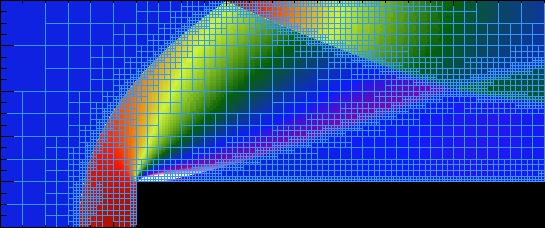
\includegraphics[width=2.5in]{paramesh2.png}}
\begin{itemize}
 \enhance{1}\item  Based on octrees rather than SAMR for scalability
\begin{itemize}
 \enhance{1}\item    octree AMR has scaled to $>$32K cores
 \enhance{1}\item    mesh data associated with leaf nodes only
\end{itemize}
 \enhance{2}\item Enhancements to address other issues
\begin{itemize}
 \enhance{2}\item   \textbf{patch coalescing} to reduce AMR overhead
 \enhance{2}\item   \textbf{targeted refinement} for deep AMR problems
\end{itemize}
\end{itemize}
\end{frame}

% \begin{frame}[fragile] 
% %--------------------------------------------------
% \frametitle{Scalability of AMR variants}
% \framesubtitle{Structured AMR}
% %--------------------------------------------------
% \includegraphics<1>[width=1.2in]{chombo.png}
% \begin{itemize}
% \item \enhance{1}  regridding algorithm
% \begin{itemize}
% \item \enhance{1}     tradeoff between mesh quality and scaling
% \item \enhance{1}     \enzo\ favors speed
% \end{itemize}
% \item \enhance{1}  variable-sized task sizes
% \begin{itemize}
% \item \enhance{1}     scheduling and load balancing
% \item \enhance{1}     performance versus parallelism
% \end{itemize}
% \item \enhance{1} neighbor searches
% \end{itemize}
% \end{frame}
% 
% \begin{frame}[fragile] 
% %--------------------------------------------------
% \frametitle{Scalability of AMR variants}
% \framesubtitle{Octree-based AMR}
% %--------------------------------------------------
% \includegraphics<1>[width=1.2in]{paramesh.png}
% \begin{itemize}
% \item \enhance{1} fixed-size patches inefficient for "shallow" AMR
% \begin{itemize}
% \item \enhance{1}  refining a single point involves entire root-level patch
% \end{itemize}
% \item \enhance{1} octree refinement inefficient for "deep" AMR
% \end{itemize}
% %       - reduced operations for physics modules compared to SAMR
% %         - cubical typically small blocks
% %         - limited inter-block configurations [ figure ]
% \end{frame}
% 
% %     - "AMR hierarchy" defines changes in resolution
% %     - "AMR patch" defines areas of uniform resolution
% %     - hierarchy size should be proportional to "amount" of resolution change

%------------------------------------------------------------------------

\begin{frame}[fragile] 
%--------------------------------------------------
\frametitle{\cello\ AMR}
\framesubtitle{Enhancement 1: Patch coalescing}
%--------------------------------------------------
\centerline{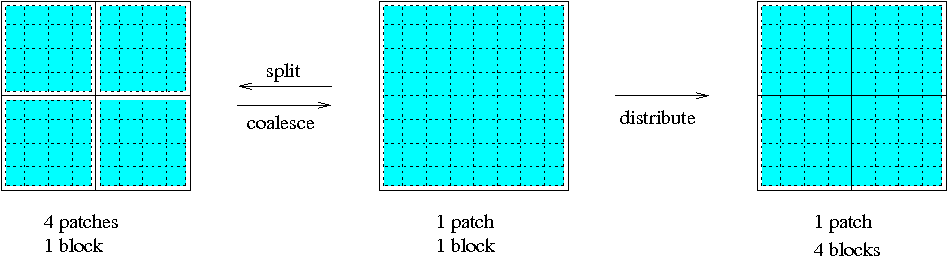
\includegraphics[width=3.5in]{coalesce2.png}}
\begin{itemize}
\enhance{2}\item Coalesce patches into larger one when possible
\enhance{3}\item Split a patch into smaller ones when necessary
\enhance{4}\item Maintain task size control using ``blocks''
\end{itemize}
\end{frame}

\begin{frame}[fragile] 
%--------------------------------------------------
\frametitle{\cello\ AMR}
\framesubtitle{Enhancement 1: Patch coalescing}
%--------------------------------------------------
\begin{minipage}{2.2in}
\includegraphics<1>[width=2.2in]{circle.png}
\includegraphics<2>[width=2.2in]{circle-1.png}
\includegraphics<3>[width=2.2in]{circle-2.png}
\end{minipage}
\begin{minipage}{1.6in}
\footnotesize
      \begin{itemize}
        \item \ENHANCE{1}Assume you want to refine on a circle
        \item \ENHANCE{2}quadtree refinement has 18517 patches
        \item \ENHANCE{3}coalescing patches reduces to 789 patches
      \end{itemize}
\end{minipage}

\end{frame}

\begin{frame}[fragile] 
%--------------------------------------------------
\frametitle{\cello\ AMR}
\framesubtitle{Enhancement 2: Targeted refinement}
%--------------------------------------------------
\centerline{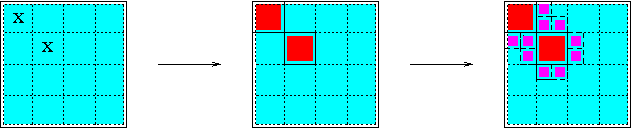
\includegraphics[width=3.5in]{kd-backfill.png}}
\begin{itemize}
\enhance{1}\item Refine by $r=4$ instead of $r=2$
\enhance{2}\item Refinement is more localized
\enhance{3}\item Can restore $r=2$ jumps by ``backfilling'' levels
\enhance{4}\item Backfill patch locations known implicitly---nominal storage
\end{itemize}
\end{frame}


\begin{frame}[fragile] 
%--------------------------------------------------
\frametitle{\cello\ AMR}
\framesubtitle{Enhancement 2: Targeted refinement}
%--------------------------------------------------
\begin{minipage}{2.2in}
\includegraphics<1>[width=2.2in]{dots-invert.png}
\includegraphics<2>[width=2.2in]{dots-4-1-inv.png}
\includegraphics<3>[width=2.2in]{dots-16-5-inv.png}
\end{minipage}
\begin{minipage}{1.6in}
\footnotesize
      \begin{itemize}
        \item \ENHANCE{1}Assume you want to refine on point sources
        \item \ENHANCE{2} quadtree refinement with $r=2$ has 2137 patches
        \item \ENHANCE{3} targeted refinement with $r=4$ has 158 patches
      \end{itemize}
\end{minipage}

\end{frame}
